\documentclass[11pt]{article}
\usepackage[a4paper,margin=1in]{geometry}
\usepackage{amsmath,amssymb,amsthm}
\usepackage{tikz}
\usepackage{xcolor}
\usepackage{booktabs}
\usepackage[hidelinks]{hyperref}
\hypersetup{pdftitle={Labelling binary trees by powers of two},pdfauthor={Vamshi Jandhyala}}
\setlength{\parskip}{0.4em}
\setlength{\parindent}{0pt}

\newtheorem{theorem}{Theorem}
\newtheorem{lemma}[theorem]{Lemma}
\newtheorem{corollary}[theorem]{Corollary}
\newtheorem{proposition}[theorem]{Proposition}
\theoremstyle{remark}
\newtheorem*{remark}{Remark}

\definecolor{inkblue}{RGB}{40,76,105}
\definecolor{rust}{RGB}{153,70,45}

\title{Labelling binary trees by powers of two}
\author{Vamshi Jandhyala}
\date{}

\begin{document}
\maketitle
\vspace{-2em}

\begin{abstract}
Can every rooted tree with $n$ vertices, each vertex having at most two children, be labelled
by $0,1,\dots,n-1$ so that the root gets $0$ and every child exceeds its parent by a power of
two? The question was asked on MathOverflow in 2018 and is still open. This note collects what
is now known. Five constructions build a labelling of a tree from labellings of smaller trees,
so a smallest counterexample must avoid all of them. A label set that works for every tree of
its size, a universal set, has a universal tail, and this turns the family of universal sets
into something that can be computed exactly: it is irregular, with sporadic members at sizes
$4,5,6,8,9,14,16,\dots,21$. Every tree with at most $24$ vertices has a labelling, and from
$11$ vertices on no proof can label the two branches of the root independently of each other's
shape. The constructions and the lemmas on universal sets are checked in the Lean proof
assistant.
\end{abstract}

\section{The question}

Take a rooted tree in which each vertex has at most two children; the children are not ordered.
Label its $n$ vertices with $0,1,\dots,n-1$, each used once, so that the root has label $0$ and
each child's label is its parent's label plus a power of two ($1,2,4,8,\dots$). Gro-Tsen asked
on MathOverflow~\cite{MO} whether this is always possible, a question that came from a
bioinformatician. Experiments say yes; nobody knows why.

Stop and try a small case before reading on. Figure~\ref{fig:example} shows one answer for a tree
with nine vertices. Every edge carries a difference of $1$, $2$ or $4$.

\begin{figure}[ht]
\centering
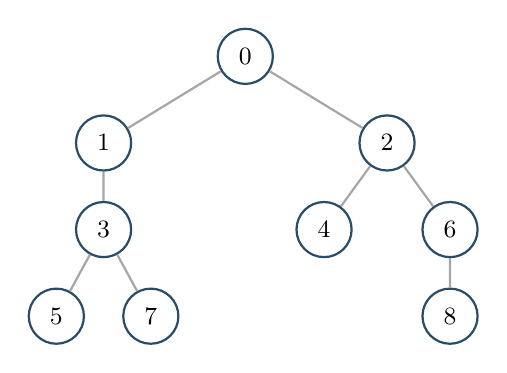
\begin{tikzpicture}[level distance=11mm,
  every node/.style={circle,draw=inkblue,thick,minimum size=7mm,inner sep=0pt,font=\small},
  edge from parent/.style={draw=gray!70,thick},
  level 1/.style={sibling distance=36mm}, level 2/.style={sibling distance=16mm},
  level 3/.style={sibling distance=12mm}]
\node {0}
  child {node {1} child {node {3} child {node {5}} child {node {7}}}}
  child {node {2} child {node {4}} child {node {6} child {node {8}}}};
\end{tikzpicture}
\caption{A labelling of a nine-vertex tree. Down the left: $1,2,2,4$; down the right: $2,2,4,2$.}
\label{fig:example}
\end{figure}

Gro-Tsen's reformulation explains the difficulty. On $\{0,\dots,n-1\}$ draw an arrow from $i$ to
$j$ whenever $j-i$ is a power of two. The question asks whether this graph, which has only about
$n\log_2 n$ arrows, contains every rooted binary tree on $n$ vertices as a spanning tree. Graphs
that contain all spanning trees of a class are studied in~\cite{CG}; Gro-Tsen saw no way to
adapt those methods to this particular graph.

Call a tree \emph{labelled} when it has such a labelling. Two simple moves keep a labelling
valid: adding a constant to every label, and doubling every label. Doubling turns each power of
two into a larger one.

\section{Building labellings from smaller ones}

Write $|T|$ for the number of vertices of $T$. A \emph{chain of $d$ vertices above} a tree $C$ is
a path $u_1,\dots,u_d$ in which each $u_i$ has the single child $u_{i+1}$, and $u_d$ has the root
of $C$ as its single child.

\begin{theorem}\label{thm:reductions}
Let $T$ be a tree and suppose that every tree named below is labelled. Then $T$ is labelled in
each of these cases.
\begin{enumerate}
\item[(a)] The root of $T$ has one child.
\item[(b)] The root has branches $A$ and $B$ with $|A|=|B|$ or $|A|=|B|+1$.
\item[(c)] The root has branches $A$, $B$ with $|A|=2^k-1$.
\item[(d)] The root has branches $A$, $B$, where $A$ is a chain of $d\ge1$ vertices above $C$, and
either $|C|\in\{|B|,|B|+1\}$ and $d+2$ is a power of two, or $|B|\in\{|C|,|C|+1\}$ and $d+1$ is
a power of two.
\item[(e)] The root has branches $A$, $B$, where $A$ is a chain of $d\ge1$ vertices above $C$, $B$ is
a chain of $e\ge1$ vertices above $D$, $d+1$ is a power of two, and either $|C|\in\{|D|,|D|+1\}$
and $e+1$ is a power of two, or $|D|\in\{|C|,|C|+1\}$ and $e+2$ is a power of two.
\end{enumerate}
\end{theorem}

Machacek's answer to the question~\cite{MOa} contains (b) for $|A|=|B|$ and (c); the cases
$|A|=|B|+1$ of (b), and (d) and (e), were found during this work (see the acknowledgements).

\begin{proof}
In each case the root gets $0$, and the labellings of the smaller trees are moved by doubling and
shifting.

(a) Label the child's subtree by its own labelling plus $1$.

(b) Put $1+2\alpha$ on $A$ and $2+2\beta$ on $B$, where $\alpha$, $\beta$ are labellings of $A$
and $B$ (Figure~\ref{fig:parity}). The branch $A$ takes the odd numbers $1,3,\dots,2|A|-1$ and
$B$ the even numbers $2,4,\dots,2|B|$; since $|A|$ is $|B|$ or $|B|+1$, together they fill
$1,\dots,|A|+|B|$ with no gap. The root's children get $1$ and $2$, and doubling keeps every
other difference a power of two.

(c) Put $\alpha+1$ on $A$, filling $1,\dots,2^k-1$, and $\beta+2^k$ on $B$. The root's children
get $1$ and $2^k$.

(d) Label the chain $1,\dots,d$. In the first case put $d+1+2\gamma$ on $C$ and $d+2+2\beta$ on
$B$: the chain ends at $d$, so the edge into $C$ has difference $1$, and the root's edge into $B$
has difference $d+2$. In the second case exchange the offsets: $d+2+2\gamma$ on $C$ and
$d+1+2\beta$ on $B$, with differences $2$ and $d+1$. In both cases the two interleaved sets fill
$d+1,\dots,d+|B|+|C|$, because the set with the smaller offset is the larger one or the same size.

(e) Put $D'=d+e$. Label the first chain $1,\dots,d$ and the second $d+1,\dots,D'$, so the root's
edges have differences $1$ and $d+1$. In the first case put $D'+1+2\gamma$ on $C$ and
$D'+2+2\delta$ on $D$; the edges from the ends of the chains have differences $e+1$ and $2$. In
the second case exchange the offsets; the differences become $e+2$ and $1$.
\end{proof}

\begin{figure}[ht]
\centering
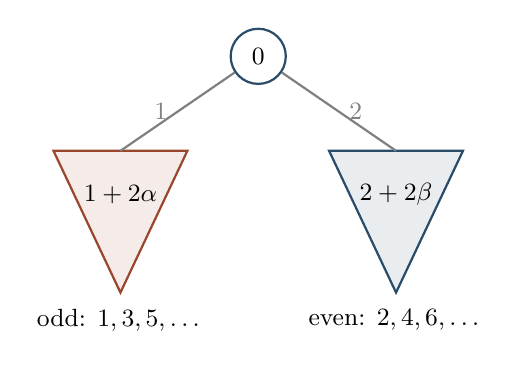
\begin{tikzpicture}[every node/.style={font=\small}]
\node[circle,draw=inkblue,thick,minimum size=7mm] (r) at (0,0) {0};
\draw[thick,draw=rust,fill=rust!10] (-2.6,-1.2) -- (-0.9,-1.2) -- (-1.75,-3.0) -- cycle;
\draw[thick,draw=inkblue,fill=inkblue!10] (0.9,-1.2) -- (2.6,-1.2) -- (1.75,-3.0) -- cycle;
\draw[thick,gray] (r) -- (-1.75,-1.2) node[midway,left] {$1$};
\draw[thick,gray] (r) -- (1.75,-1.2) node[midway,right] {$2$};
\node at (-1.75,-1.75) {$1+2\alpha$};
\node at (1.75,-1.75) {$2+2\beta$};
\node at (-1.75,-3.35) {odd: $1,3,5,\dots$};
\node at (1.75,-3.35) {even: $2,4,6,\dots$};
\end{tikzpicture}
\caption{Theorem~\ref{thm:reductions}(b): branches whose sizes differ by at most one share out the
odd and the even labels.}
\label{fig:parity}
\end{figure}

So a smallest tree without a labelling has a root with two children, branch sizes that differ by
at least two, neither branch of size $2^k-1$, and none of the chain shapes of (d) and (e).

\section{Universal label sets}

The constructions above all label the branches with sets of a special form. It is natural to ask
which sets can serve every tree of a given size. Call a finite set $S$ of natural numbers with
$0\in S$ \emph{universal} if every tree with $|S|$ vertices has a labelling onto $S$ (a bijection
with root $0$ and each child exceeding its parent by a power of two). The question asks whether
each interval $\{0,\dots,n-1\}$ is universal. Call $S$ \emph{primitive} if it contains an odd
number. For example, $\{0,2,3,4\}$ is universal: each of the three trees with four vertices
can be labelled onto it.

\begin{lemma}[tail lemma]\label{lem:tail}
Let $S$ be universal with $|S|\ge2$, and let $p$ be its smallest positive element. Then $p$ is a
power of two and $T=\{s-p:s\in S,\ s>0\}$ is universal.
\end{lemma}

\begin{proof}
Let $U$ be any tree with $|S|-1$ vertices, and put a new root with $U$ as its only child. A
labelling of this tree onto $S$ gives the new root $0$. Every other vertex descends from the
root's child, and labels increase along every edge, so the child gets the smallest positive
label $p$, and $p-0$ is a power of two. Subtracting $p$ from the labels of $U$ gives a labelling
of $U$ onto $T$.
\end{proof}

\begin{lemma}[primitive tail]\label{lem:prim}
If moreover $S$ is primitive and $|S|\ge3$, then $T$ is primitive and some element of $T$ is at
least $p$.
\end{lemma}

\begin{proof}
A root with two children, one a leaf, is a tree with $|S|$ vertices, so $S$ contains the labels
of two children of $0$: two different powers of two. One of them, $q$, differs from $p$, and
since $p$ is the least positive element, $q>p$, so $q\ge2p$ and $q-p\in T$ is at least $p$.
If every element of $T$ were even, then either $p\ge2$ is even and every element of $S$ is even,
or $p=1$ and every positive element of $S$ is odd, which leaves no room for the even power of two
$q$. Both contradict the hypotheses.
\end{proof}

So every primitive universal set with $n\ge3$ elements has the form
\begin{equation}\label{eq:gen}
S=\{0\}\cup(p+T),\qquad T \text{ primitive universal},\ |T|=n-1,\ p \text{ a power of two},\ p\le\max T.
\end{equation}
Read it as: $S$ is a primitive universal set one size smaller, lifted by a power of two that is
not too large, with $0$ added. Only finitely many candidates arise at each size, and testing each
candidate against every tree finds all primitive universal sets of the next size exactly, with no
assumed bound on how large the labels can be. Induction on~\eqref{eq:gen} also bounds them.

\begin{corollary}\label{cor:span}
A primitive universal set with $n\ge2$ elements lies in $\{0,1,\dots,2^{n-2}\}$.
\end{corollary}

\begin{proof}
For $n=2$ the set is $\{0,p\}$ with $p$ an odd power of two, so $p=1$. For larger $n$, every
element of $S$ is $0$ or $p+t$ with $t\in T$, and $p$ is at most an element of $T$; both are at
most $2^{n-3}$ by induction, so $p+t\le2^{n-2}$.
\end{proof}

Running the rule to size $21$ gives Table~\ref{tab:univ}. The intervals are always there, as the
question predicts for $n\le24$ (Section~\ref{sec:comp}). The other members appear and disappear
with no visible pattern.

\begin{table}[ht]
\centering
\begin{tabular}{rl}
\toprule
$n$ & primitive universal sets other than $\{0,\dots,n-1\}$, written as $[0,m]$ minus a set\\
\midrule
4 & $[0,4]\setminus\{1\}$\\
5 & $[0,5]\setminus\{2\}$,\quad $[0,6]\setminus\{1,3\}$\\
6 & $[0,6]\setminus\{3\}$\\
8 & $[0,8]\setminus\{1\}$\\
9 & $[0,10]\setminus\{1,3\}$\\
14 & $[0,14]\setminus\{1\}$\\
16 & $[0,16]\setminus\{1\}$,\quad $[0,18]\setminus\{1,2,3\}$\\
17 & $[0,17]\setminus\{2\}$,\quad $[0,18]\setminus\{1,3\}$\\
18 & $[0,18]\setminus\{3\}$,\quad $[0,20]\setminus\{1,3,5\}$\\
19 & $[0,19]\setminus\{1\}$,\quad $[0,19]\setminus\{4\}$,\quad $[0,22]\setminus\{1,3,5,7\}$\\
20 & $[0,20]\setminus\{2\}$,\quad $[0,20]\setminus\{5\}$\\
21 & $[0,21]\setminus\{3\}$,\quad $[0,21]\setminus\{6\}$\\
\bottomrule
\end{tabular}
\caption{Every primitive universal set of size $n\le21$ that is not an interval. Sizes not listed
($n\le21$) have the interval only.}
\label{tab:univ}
\end{table}

\section{Computations}\label{sec:comp}

\begin{proposition}\label{prop:comp}
\begin{enumerate}
\item[(i)] Every tree with at most $24$ vertices is labelled.
\item[(ii)] Every tree with at most $22$ vertices has a labelling in which the root's children get
$1$ and $2$ (or $1$, for a single child).
\item[(iii)] Table~\ref{tab:univ} lists every primitive universal set of size at most $21$.
\item[(iv)] For $n\le11$, the only split of $n-1$ vertices into branch sizes $a\ge b$ for which no
pair of sets $p+S_1$, $q+S_2$ (with $p\ne q$ powers of two, $S_1$, $S_2$ universal sets of sizes
$a$, $b$, possibly doubled) partitions $\{1,\dots,n-1\}$ is $(6,4)$.
\end{enumerate}
\end{proposition}

These are exhaustive searches, and the folder of this note holds the programs. For (i), one
program checks all $34{,}504{,}201$ trees with at most $24$ vertices, using
Theorem~\ref{thm:reductions} for the $26$ million that it covers and searching the rest; a
second, separately written program checks every tree up to $22$ vertices; a third, in Python,
searches every tree up to $12$ vertices with no reductions. For (ii), one program searches every
tree up to $22$ vertices directly, and the Python program rechecks up to $12$. For (iii), two
separately written programs generate the sets by~\eqref{eq:gen} and agree up to size $20$; one
of them continues to $21$; the Python program rechecks up to $9$. Part (iv) is checked by the
Python program.

Part (iv) says something about proofs. A proof by induction on the size of the tree would like to
label the two branches of the root by fixed universal sets, chosen from the branch sizes alone,
so that the induction hypothesis applies to each branch separately. Up to $10$ vertices that
works. At $11$ vertices, with branches of sizes $6$ and $4$, no such choice exists, so an
inductive proof has to let the label set of one branch depend on the shape of the other.

\section*{Data and code}
The programs, their outputs and an independent Python check of every finite statement are in
the folder of this note at \url{https://github.com/jvvk/mathematics}. Theorem~\ref{thm:reductions},
Lemmas~\ref{lem:tail} and~\ref{lem:prim} and Corollary~\ref{cor:span} are checked in the Lean
proof assistant.

\section*{Acknowledgements}
The constructions in Theorem~\ref{thm:reductions} beyond Machacek's, the second labelling
program, the program for Proposition~\ref{prop:comp}(ii) and the second program for (iii) were
found or written with Codex (OpenAI); the tail lemma, the remaining programs, the Lean proofs and
this text were developed with Claude (Anthropic), all under the author's direction. The author
thanks Gro-Tsen for the question and John Machacek and Gerhard Paseman for their answers. The
author is responsible for the contents.

\begin{thebibliography}{9}
\bibitem{CG} F.~R.~K.~Chung and R.~L.~Graham, On universal graphs for spanning trees,
\emph{J. London Math. Soc.} (2) \textbf{27} (1983) 203--211,
\href{https://doi.org/10.1112/jlms/s2-27.2.203}{doi:10.1112/jlms/s2-27.2.203}.
\bibitem{MO} Gro-Tsen, Labeling binary trees so that adjacent vertices differ by a power of two,
MathOverflow question 304266 (2018), \url{https://mathoverflow.net/q/304266}, accessed 10 October
2026.
\bibitem{MOa} J.~Machacek, answer to~\cite{MO}, \url{https://mathoverflow.net/a/304271}, accessed
10 October 2026.
\end{thebibliography}

\end{document}
